%\chapter{Limits of Random Variables}


\chapter{Limit Laws of Statistics}\label{S:LimitLawsStats}

\begin{prop}[Central Limit Theorem (CLT)]
Let $X_1,X_2,\ldots \overset{\IID}{\sim} X_1$ and suppose $\e(X_1)$ and $\V(X_1)$ exists, then 
{\small
\begin{eqnarray}
%1
\overline{X}_n = \frac{1}{n} \sum_{i=1}^n X_i 
& \rightsquigarrow & 
X \sim \normal \left( \e(X_1),\frac{\V(X_1)}{n}  \right) \ , \\
%2
\overline{X}_n -\e(X_1) 
& \rightsquigarrow & 
X-\e(X_1) \sim \normal \left( 0,\frac{\V(X_1)}{n}  \right) \ , \\
%3
\sqrt{n} \left( \overline{X}_n -\e(X_1) \right)
& \rightsquigarrow & 
\sqrt{n} \left( X-\e(X_1) \right) \sim \normal \left( 0,\V(X_1)  \right) \ , \\
%4
Z_n :=  \frac{\overline{X}_n-\e(\overline{X}_n)}{\sqrt{\V(\overline{X}_n)}} 
= \frac{\sqrt{n} \left( \overline{X}_n -\e(X_1) \right)}{\sqrt{\V(X_1)}}
& \rightsquigarrow & 
Z  \sim \normal \left( 0,1  \right) \ , \\
%5
\lim_{n \to \infty} P\left( \frac{\overline{X}_n-\e(\overline{X}_n)}{\sqrt{\V(\overline{X}_n)}}  \leq z \right)
= \lim_{n \to \infty} \p(Z_n \leq z)
&=&
\Phi(z) := \int_{- \infty}^z \left( \frac{1}{\sqrt{2 \pi}} \ \exp \left( \frac{-x^2}{2} \right) \right) dx \ .
\end{eqnarray}
}
Thus, for sufficiently large $n$ (say $n>30$) we can make the following approximation:
\begin{equation}\label{E:CLTApprox}
P\left( \frac{\overline{X}_n-\e(\overline{X}_n)}{\sqrt{\V(\overline{X}_n)}}  \leq z \right) 
\approxeq 
\p(Z \leq z)
=
\Phi(z) := \int_{- \infty}^z \left( \frac{1}{\sqrt{2 \pi}} \ \exp \left( \frac{-x^2}{2} \right) \right) dx \ .
\end{equation}
{\scriptsize
\begin{proof}
See any intermediate to advanced undergraduate text in Probability.  Start from the index looking for ``Central Limit Theorem'' to find the page number for the proof \ldots .
\end{proof}
}
{\bf Heuristic Interpretation of CLT:}  Probability statements about the sample mean RV $\overline{X}_n$ can be approximated using a Normal distribution. 
\end{prop}
Here is a simulation showing CLT in action.
\begin{VrbM}
>> % a demonstration of Central Limit Theorem --
>> % the sample mean of a sequence of n IID Exponential(lambda) RVs 
>> % itself a Gaussian(1/lambda,lambda/n) RV
>> lambda=0.1; Reps=10000; n=10; hist(sum(-1/lambda * log(rand(n,Reps)))/n)
>> lambda=0.1; Reps=10000; n=100; hist(sum(-1/lambda * log(rand(n,Reps)))/n,20)
>> lambda=0.1; Reps=10000; n=1000; hist(sum(-1/lambda * log(rand(n,Reps)))/n,20)
\end{VrbM}

Let us look at an example that makes use of the CLT next.
\begin{example}[Errors in computer code (Wasserman03, p.~78)]\label{EX:CLTPoisson}
Suppose the collection of RVs $X_1,X_2, \ldots, X_n$ model the number of errors in $n$ computer programs named $1,2,\ldots,n$, respectively.  Suppose that the RV $X_i$ modeling the number of errors in the $i$-th program is the $Poisson(\lambda=5)$ for any $i=1,2,\ldots,n$.  Further suppose that they are independently distributed.  Succinctly, we suppose that 
\[
X_1,X_2,\ldots,X_n \overset{\IID}{\sim} \poisson(\lambda=5) \ . 
\]
Suppose we have $n=125$ programs and want to make a probability statement about $\overline{X}_n$ which is the average error per program out of these $125$ programs.  Since $\e(X_i) = \lambda=5$ and $\V(X_i)=\lambda=5$, we may want to know how often our sample mean $\overline{X}_{125}$ differs from the expectation of $5$ errors per program.  Using the CLT we can approximate $\p(\overline{X}_n < 5.5)$, for instance, as follows:
\begin{eqnarray}
\p(\overline{X}_n < 5.5) 
&=& P \left( \frac{\sqrt{n}(\overline{X}_n - \e(X_1))}{\sqrt{\V(X_1)}} < \frac{\sqrt{n}(5.5-\e(X_1))}{\sqrt{\V(X_1)}} \right) \notag \\
&\approxeq& P \left( Z < \frac{\sqrt{n}(5.5-\lambda)}{\sqrt{\lambda}} \right) \qquad \text{{\scriptsize [by \eqref{E:CLTApprox}, and $\e(X_1)=\V(X_1)=\lambda$]}} \notag \\
&=& P \left( Z < \frac{\sqrt{125}(5.5-5)}{\sqrt{5}} \right) \qquad \text{{\scriptsize [Since, $\lambda=5$ and $n=125$ in this Example]}} \notag \\
&=& \p(Z \leq 2.5) = \Phi(2.5) =  \int_{- \infty}^{2.5} \left( \frac{1}{\sqrt{2 \pi}} \ \exp \left( \frac{-x^2}{2} \right) \right) dx \approxeq 0.993790334674224 \ . \notag
\end{eqnarray}
The last number above needed the following:
\begin{labwork}[Numerical approximation of $\Phi(2.5)$]
The numerical approximation of $\Phi(2.5)$ was obtained via the following call to our $\erf$-based {\tt NormalCdf} function. % from \ref*{Mf: NormalCdfPdf}. MATLABback
\begin{VrbM}
>> format long
>> disp(NormalCdf(2.5,0,1))
   0.993790334674224
\end{VrbM}
\end{labwork}
\end{example}
The CLT says that if $X_1,X_2,\ldots \overset{\IID}{\sim} X_1$, then $Z_n := \sqrt{n}(\overline{X}_n-\e(X_1))/\sqrt{\V(X_1)}$ is approximately distributed as $\normal(0,1)$.  In \hyperref[EX:CLTPoisson]{Example \ref*{EX:CLTPoisson}}, we knew $\sqrt{\V(X_1)}$.   However, in general, we may not know $\sqrt{\V(X_1)}$.  The next proposition says that we may estimate $\sqrt{\V(X_1)}$ using the sample standard deviation $S_n$ of $X_1,X_2,\ldots,X_n$, according to \eqref{E:SampleStdDevRV}, and still make probability statements about the sample mean $\overline{X}_n$ using a Normal distribution.
\begin{prop}[CLT based on Sample Variance]
Let $X_1,X_2,\ldots \overset{\IID}{\sim} X_1$ and suppose $\e(X_1)$ and $\V(X_1)$ exists, then
\begin{equation}\label{E:CLTApproxSn}
\frac{\sqrt{n} \left( \overline{X}_n - \e(X_1) \right)}{S_n} \rightsquigarrow \normal(0,1) \ .
\end{equation}
\end{prop}

We will use \eqref{E:CLTApproxSn} for statistical estimation in the sequel.

%The next proposition is often referred to as the fundamental theorem of statistics and is at the heart of non-parametric inference, empirical processes, and computationally-intensive bootstrap techniques.
%\begin{prop}[Gilvenko-Cantelli Theorem]\label{P:Gilvenko-Cantelli}
%Let $X_1,X_2,\ldots,X_n \overset{\IID}{\sim} F$.  Then,
%\[
%\sup_x { | \widehat{F}_n(x) - F(x) | } \overset{P}{\longrightarrow} 0 \ .
%\]
%{\scriptsize
%\begin{proof}
%Proof to be seen in STAT 318 or another advanced Statistics course.
%\end{proof}
%}
%\end{prop}
%{\bf Heuristic Interpretation of Gilvenko-Cantelli Theorem}:  As the sample size $n$ increases the empirical distribution function $\widehat{F}_n$ converges to the true DF $F$ in probability.

%\begin{figure}[htpb]
%\caption{Plots of ten distinct ECDFs $\widehat{F}_n$ based on $10$ sets of $n$ IID samples from $\uniform(0,1)$ RV $X$, as $n$ increases from $10$ to $100$ to $1000$.  The DF $F(x)=x$ over $[0,1]$ is shown in red.  The script of \hyperref[Mf:GilvenkoCantelliUnif01n10n100n100ECDFs]{Labwork \ref*{Mf:GilvenkoCantelliUnif01n10n100n100ECDFs}} was used to generate this plot.   \label{F:GilvenkoCantelliUnif01n10n100n100ECDFs}}
%\centering   \makebox{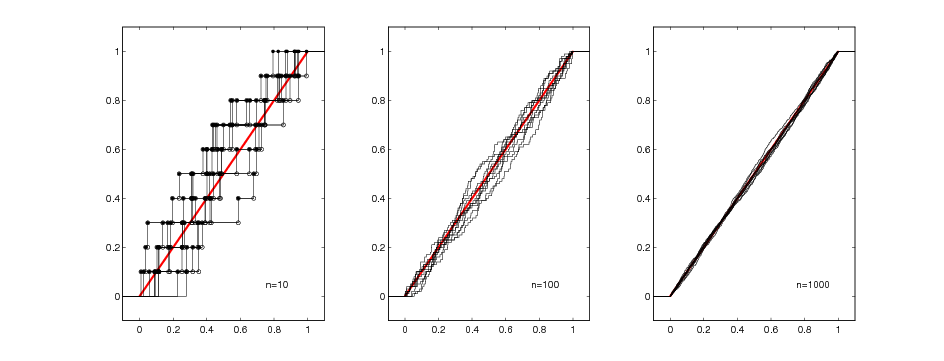
\includegraphics[width=7.0in]{figures/GilvenkoCantelliUnif01n10n100n100ECDFs}}
%\end{figure}

%\begin{prop}[The Dvoretzky-Kiefer-Wolfowitz (DKW) Inequality]
%Let $X_1,X_2,\ldots,X_n \overset{\IID}{\sim} F$.  Then, for any $\epsilon>0$,
%\begin{equation}\label{E:DKWNeq}
%P \left( \sup_x | \widehat{F}_n(x) - F(x) | > \epsilon  \right) \leq 2 \exp {(-2 n \epsilon^2)}
%\end{equation}
%\end{prop}
